\section{Subdivisión baricéntrica de un símplice}

% ------------------------------------------------------------------------
\subsection{Símplices generalizados}

\begin{frame}
  \frametitle{Símplices generalizados}

  \begin{definition}
    Dada una lista de $n+1$ puntos $v_0,\ldots,v_n\in\R^N$, el
    \alert{símplice generalizado} de dimensión $n$ y vértices
    $v_0,\ldots,v_n$ es su envolvente convexa
    \[
      [v_0,\ldots,v_n]=\Bigl\{\,t_0v_0+\cdots+t_nv_n \;:\;
      t_i\geq0,\ t_0+\cdots+t_n=1\,\Bigr\}.
    \]
    Los $(t_0,\ldots,t_n)$ son \alert{unas coordenadas baricéntricas} del punto
    $t_0v_0+\cdots+t_nv_n$.
  \end{definition}

  \medskip

  Los vértices pueden repetirse o puede haber tres alineados.
  El símplice generalizado viene dado por la
  \alert{lista} de sus vértices, en ese orden: listas distintas dan
  símplices generalizados distintos, aunque tengan la misma envolvente.
\end{frame}

\begin{frame}
  \frametitle{Símplices y símplices degenerados}

  Hay dos tipos de símplices generalizados $[v_0,\ldots,v_n]$:
  \begin{itemize}
    \item si $v_0,\ldots,v_n$ son afínmente independientes, es un
      \alert{símplice} en el sentido usual, y cada punto tiene
      coordenadas baricéntricas \alert{únicas};
    \item en otro caso, decimos que es un \alert{símplice degenerado}.
  \end{itemize}

  \medskip

  En lo que sigue, «símplice» a secas significa siempre no degenerado.
\end{frame}

\begin{frame}
  \frametitle{Ejemplos de símplices}

  \begin{columns}[T]
    \begin{column}{0.30\textwidth}
      \centering
      \begin{tikzpicture}
        \useasboundingbox (-0.5,-0.9) rectangle (2.9,2.4);
        \coordinate (A) at (0,0.6);
        \coordinate (B) at (2.4,0.6);
        \draw[thick] (A) -- (B);
        \fill (A) circle (1.6pt) node[below] {$v_0$};
        \fill (B) circle (1.6pt) node[below] {$v_1$};
      \end{tikzpicture}

      \small Un segmento $[v_0,v_1]$.
    \end{column}
    \begin{column}{0.30\textwidth}
      \centering
      \begin{tikzpicture}
        \useasboundingbox (-0.5,-0.9) rectangle (2.9,2.4);
        \coordinate (A) at (0,0);
        \coordinate (B) at (2.4,0);
        \coordinate (C) at (1.2,2);
        \filldraw[thick,fill=alertcolor!10] (A) -- (B) -- (C) -- cycle;
        \fill (A) circle (1.6pt) node[below] {$v_0$};
        \fill (B) circle (1.6pt) node[below] {$v_1$};
        \fill (C) circle (1.6pt) node[above] {$v_2$};
      \end{tikzpicture}

      \small Un triángulo $[v_0,v_1,v_2]$.
    \end{column}
    \begin{column}{0.30\textwidth}
      \centering
      \begin{tikzpicture}
        \useasboundingbox (-0.5,-0.9) rectangle (2.9,2.4);
        \coordinate (A) at (0,0.1);
        \coordinate (B) at (1.7,-0.4);
        \coordinate (C) at (2.5,0.6);
        \coordinate (D) at (1.2,2);
        \fill[alertcolor!10] (A) -- (B) -- (C) -- (D) -- cycle;
        \draw[dashed] (A) -- (C);
        \draw[thick] (A) -- (B) -- (C) -- (D) -- cycle (B) -- (D);
        \fill (A) circle (1.6pt) node[left] {$v_0$};
        \fill (B) circle (1.6pt) node[below] {$v_1$};
        \fill (C) circle (1.6pt) node[right] {$v_2$};
        \fill (D) circle (1.6pt) node[above] {$v_3$};
      \end{tikzpicture}

      \small Un tetraedro $[v_0,v_1,v_2,v_3]$.
    \end{column}
  \end{columns}

  \bigskip

  En todos ellos, coordenadas baricéntricas distintas dan puntos distintos:
  cada punto tiene coordenadas baricéntricas \alert{únicas}.
\end{frame}

\begin{frame}
  \frametitle{Ejemplos de símplices degenerados}

  \begin{columns}[T]
    \begin{column}{0.22\textwidth}
      \centering
      \begin{tikzpicture}
        \useasboundingbox (-1.1,-0.9) rectangle (1.1,2.2);
        \fill (0,0.6) circle (1.8pt) node[below=4pt] {$v_0=v_1$};
      \end{tikzpicture}

      \footnotesize
      Si $v_0=v_1$, $[v_0,v_1]$ es un punto. Todo $(t_0,t_1)$ da el mismo
      punto.
    \end{column}
    \begin{column}{0.24\textwidth}
      \centering
      \begin{tikzpicture}
        \useasboundingbox (-0.6,-0.9) rectangle (2.4,2.2);
        \coordinate (A) at (0,0.6);
        \coordinate (B) at (2,0.6);
        \draw[thick] (A) -- (B);
        \fill (A) circle (1.6pt) node[below=4pt] {$v_0=v_1$};
        \fill (B) circle (1.6pt) node[below=4pt] {$v_2$};
      \end{tikzpicture}

      \footnotesize
      Si $v_0=v_1$, $[v_0,v_1,v_2]$ es un segmento. El punto $v_0$ tiene
      coordenadas $(1,0,0)$ y $(0,1,0)$.
    \end{column}
    \begin{column}{0.24\textwidth}
      \centering
      \begin{tikzpicture}
        \useasboundingbox (-0.4,-0.9) rectangle (2.4,2.2);
        \coordinate (A) at (0,0.6);
        \coordinate (B) at (2,0.6);
        \coordinate (M) at (1,0.6);
        \draw[thick] (A) -- (B);
        \fill (A) circle (1.6pt) node[below=4pt] {$v_0$};
        \fill (B) circle (1.6pt) node[below=4pt] {$v_1$};
        \fill (M) circle (1.6pt) node[below=4pt] {$v_2$};
      \end{tikzpicture}

      \footnotesize
      Si $v_2=\frac12v_0+\frac12v_1$, $[v_0,v_1,v_2]$ es un segmento.
      El punto $v_2$ tiene coordenadas $(0,0,1)$ y $(\frac12,\frac12,0)$.
    \end{column}
    \begin{column}{0.24\textwidth}
      \centering
      \begin{tikzpicture}
        \useasboundingbox (-0.5,-0.9) rectangle (2.5,2.2);
        \coordinate (A) at (0,0);
        \coordinate (B) at (2,0);
        \coordinate (C) at (2.2,1.6);
        \coordinate (D) at (0.3,1.4);
        \filldraw[thick,fill=alertcolor!10] (A) -- (B) -- (C) -- (D) -- cycle;
        \fill (A) circle (1.6pt) node[below] {$v_0$};
        \fill (B) circle (1.6pt) node[below] {$v_1$};
        \fill (C) circle (1.6pt) node[above] {$v_2$};
        \fill (D) circle (1.6pt) node[above] {$v_3$};
      \end{tikzpicture}

      \footnotesize
      Con vértices coplanarios, $[v_0,v_1,v_2,v_3]$ es un cuadrilátero, de dimensión $3$
      como símplice generalizado.
    \end{column}
  \end{columns}
\end{frame}

\begin{frame}
  \frametitle{Caras y diámetro}

  \begin{definition}
    Sea $\sigma=[v_0,\ldots,v_n]$ un símplice generalizado con $n\geq1$. Su
    \alert{cara $i$-ésima} es el símplice generalizado de dimensión $n-1$
    \[
      \partial_i\sigma=[v_0,\ldots,\widehat{v_i},\ldots,v_n],
      \qquad 0\leq i\leq n,
    \]
    obtenido al suprimir el vértice $v_i$.

    \medskip

    El \alert{diámetro} de $\sigma$ es
    \[
      \diam\sigma=\sup\{\,|x-y| : x,y\in\sigma\,\}.
    \]
  \end{definition}

  \medskip

  Cada cara está contenida en $\sigma$, luego
  $\diam \partial_i\sigma\leq\diam\sigma$. Las caras de un símplice son símplices;
  las de un símplice degenerado pueden serlo o no.
\end{frame}

% ------------------------------------------------------------------------
\subsection{Baricentro y subdivisión}

\begin{frame}
  \frametitle{El baricentro}

  \begin{definition}
    El \alert{baricentro} del símplice generalizado $\sigma=[v_0,\ldots,v_n]$
    es el punto de coordenadas baricéntricas
    $\bigl(\frac{1}{n+1},\ldots,\frac{1}{n+1}\bigr)$:
    \[
      b_\sigma=\frac{1}{n+1}\,(v_0+v_1+\cdots+v_n)\in\sigma.
    \]
  \end{definition}

  \begin{columns}[c]
    \begin{column}{0.58\textwidth}
      Aunque se pierda la unicidad de las coordenadas, el baricentro
      tiene sentido. Depende de la \alert{lista} de vértices, no solo de la
      envolvente: $[a,b]$ y $[a,a,b]$ son el mismo segmento, pero
      \[
        b_{[a,b]}=\tfrac12a+\tfrac12b,
        \qquad
        b_{[a,a,b]}=\tfrac23a+\tfrac13b.
      \]
    \end{column}
    \begin{column}{0.38\textwidth}
      \centering
      \begin{tikzpicture}
        \coordinate (A) at (0,0);
        \coordinate (B) at (3.6,0);
        \draw[thick] (A) -- (B);
        \fill (A) circle (1.6pt) node[below] {$a$};
        \fill (B) circle (1.6pt) node[below] {$b$};
        \fill[alertcolor] (1.8,0) circle (1.6pt)
          node[above] {$b_{[a,b]}$};
        \fill[alertcolor] (1.2,0) circle (1.6pt)
          node[below] {$b_{[a,a,b]}$};
      \end{tikzpicture}
    \end{column}
  \end{columns}
\end{frame}

\begin{frame}
  \frametitle{La subdivisión baricéntrica}

  \begin{definition}
    La \alert{subdivisión baricéntrica} de un símplice generalizado
    $\sigma$ de dimensión $n$ es la familia finita $\sd(\sigma)$ de
    símplices generalizados de dimensión $n$ definida por recurrencia en
    $n$:
    \begin{itemize}
      \item si $n=0$, $\sd(\sigma)=\{\sigma\}$;
      \item si $n\geq1$, $\sd(\sigma)$ está formada por los
        \[
          [b_\sigma,w_0,\ldots,w_{n-1}]
          \quad\text{con}\quad
          [w_0,\ldots,w_{n-1}]\in\sd(\partial_i\sigma),\ 0\leq i\leq n.
        \]
    \end{itemize}
  \end{definition}

  \medskip

  Es decir, se subdividen las caras y se hace el \alert{cono} desde el
  baricentro sobre cada símplice generalizado obtenido. En la familia puede
  haber repeticiones si $\sigma$ es degenerado.
\end{frame}

\begin{frame}
  \frametitle{Ejemplos}

  \begin{columns}[T]
    \begin{column}{0.36\textwidth}
      \centering
      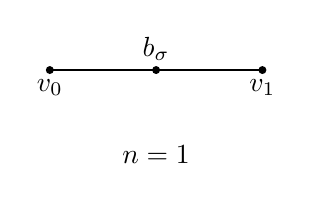
\begin{tikzpicture}[scale=0.9]
        \coordinate (A) at (0,0);
        \coordinate (B) at (3,0);
        \coordinate (M) at (1.5,0);
        \draw[thick] (A) -- (B);
        \foreach \p/\l/\pos in {A/v_0/below, B/v_1/below, M/b_\sigma/above}
          \fill (\p) circle (1.6pt) node[\pos] {$\l$};
        \node at (1.5,-1.2) {$n=1$};
      \end{tikzpicture}

      \medskip

      \small
      Si $n=1$, $\sd[v_0,v_1]=\{[b_\sigma,v_1],[b_\sigma,v_0]\}$.
    \end{column}
    \begin{column}{0.60\textwidth}
      \centering
      \begin{tikzpicture}[scale=0.9]
        \coordinate (A) at (0,0);
        \coordinate (B) at (4,0);
        \coordinate (C) at (2,3.3);
        \coordinate (G) at ($1/3*(A)+1/3*(B)+1/3*(C)$);
        \draw (G) -- (A) (G) -- (B) (G) -- (C);
        \draw (G) -- ($(A)!0.5!(B)$) (G) -- ($(B)!0.5!(C)$)
              (G) -- ($(C)!0.5!(A)$);
        \draw[thick] (A) -- (B) -- (C) -- cycle;
        \foreach \p in {A,B,C,G}
          \fill (\p) circle (1.6pt);
        \foreach \p/\q in {A/B,B/C,C/A}
          \fill ($(\p)!0.5!(\q)$) circle (1.3pt);
        \node[below left] at (A) {$v_0$};
        \node[below right] at (B) {$v_1$};
        \node[above] at (C) {$v_2$};
        \node[left=5pt] at (G) {$b_\sigma$};
      \end{tikzpicture}

      \small
      Si $n=2$, hay seis triángulos $[b_\sigma,b_{\partial_i\sigma},v_j]$ con $j\neq i$.
    \end{column}
  \end{columns}

  \medskip

  En general $\sd(\sigma)$ tiene $(n+1)!$ elementos, y si $\sigma$ es un
  símplice, estos son símplices y recubren $\sigma$. No usaremos estos
  hechos.
\end{frame}

% Dibuja la subdivisión baricéntrica del triángulo de vértices #1, #2, #3.
% Se define fuera del frame: Beamer no admite # en el cuerpo de un frame.
\newcommand{\subdividir}[3]{%
  \coordinate (g) at ($1/3*(#1)+1/3*(#2)+1/3*(#3)$);
  \draw[very thin] (g) -- (#1) (g) -- (#2) (g) -- (#3)
    (g) -- ($(#1)!0.5!(#2)$) (g) -- ($(#2)!0.5!(#3)$)
    (g) -- ($(#3)!0.5!(#1)$);}

\begin{frame}
  \frametitle{Subdivisión iterada}

  \begin{definition}
    Para $k\geq0$ definimos $\sd^0(\sigma)=\{\sigma\}$ y
    \[
      \sd^{k+1}(\sigma)=\bigcup_{\tau\in\sd^k(\sigma)}\sd(\tau).
    \]
  \end{definition}

  \begin{center}
    \begin{tikzpicture}[scale=0.85]
      \coordinate (A) at (0,0);
      \coordinate (B) at (4,0);
      \coordinate (C) at (2,3.3);
      \coordinate (G) at ($1/3*(A)+1/3*(B)+1/3*(C)$);
      \coordinate (AB) at ($(A)!0.5!(B)$);
      \coordinate (BC) at ($(B)!0.5!(C)$);
      \coordinate (CA) at ($(C)!0.5!(A)$);
      \subdividir{G}{A}{AB}
      \subdividir{G}{AB}{B}
      \subdividir{G}{B}{BC}
      \subdividir{G}{BC}{C}
      \subdividir{G}{C}{CA}
      \subdividir{G}{CA}{A}
      \draw (G) -- (A) (G) -- (B) (G) -- (C) (G) -- (AB) (G) -- (BC)
        (G) -- (CA);
      \draw[thick] (A) -- (B) -- (C) -- cycle;
    \end{tikzpicture}
  \end{center}

  \centering
  $\sd^2(\sigma)$ para un triángulo: los símplices se hacen
  \alert{cada vez más pequeños}.
\end{frame}

% ------------------------------------------------------------------------
\subsection{El diámetro de la subdivisión}

\begin{frame}
  \frametitle{La subdivisión está dentro de $\sigma$}

  \begin{lemma}
    Si $\tau\in\sd(\sigma)$, entonces $\tau\subseteq\sigma$.
  \end{lemma}

  \begin{proof}
    Como $\tau$ es la envolvente convexa de sus vértices, basta ver que los
    vértices de $\tau$ están en el convexo $\sigma$. Razonamos por
    inducción en $n$; el caso $n=0$ es trivial.

    \medskip

    Si $n\geq1$, entonces $\tau=[b_\sigma,w_0,\ldots,w_{n-1}]$ con
    $[w_0,\ldots,w_{n-1}]\in\sd(\partial_i\sigma)$. Ya sabemos que
    $b_\sigma\in\sigma$. Por hipótesis de inducción, cada $w_j$ está en
    $\partial_i\sigma$, que está contenida en $\sigma$.
  \end{proof}

  Por inducción en $k$, lo mismo vale para todo $\tau\in\sd^k(\sigma)$.
\end{frame}

\begin{frame}
  \frametitle{El diámetro lo determinan los vértices}

  \begin{lemma}
    Sea $\sigma=[v_0,\ldots,v_n]$. Para todo $p\in\R^N$ y todo
    $x\in\sigma$,
    \[
      |x-p|\leq\max_j|v_j-p|.
    \]
    En consecuencia, $\diam\sigma=\max_{i,j}|v_i-v_j|$.
  \end{lemma}

  \begin{proof}
    Si $x=\sum_jt_jv_j$ con $t_j\geq0$ y $\sum_jt_j=1$, entonces
    \[
      |x-p|=\Bigl|\sum_jt_j(v_j-p)\Bigr|
      \leq\sum_jt_j|v_j-p|
      \leq\max_j|v_j-p|.
    \]
    Si $x,y\in\sigma$, aplicando esto con $p=y$ y luego con $p=v_j$ se
    obtiene $|x-y|\leq\max_j|v_j-y|\leq\max_{i,j}|v_i-v_j|$. La
    desigualdad contraria se da porque los vértices están en $\sigma$.
  \end{proof}
\end{frame}

\begin{frame}
  \frametitle{Distancia al baricentro}

  \begin{lemma}
    Sea $\sigma=[v_0,\ldots,v_n]$. Para todo $x\in\sigma$,
    \[
      |x-b_\sigma|\leq\frac{n}{n+1}\diam\sigma.
    \]
  \end{lemma}

  \begin{proof}
    Por el lema anterior con $p=b_\sigma$, basta probarlo para los vértices $x=v_i$.
    Como
    \[
      v_i-b_\sigma=\frac{1}{n+1}\sum_{j=0}^n(v_i-v_j)
    \]
    y el sumando $j=i$ es nulo, quedan a lo sumo $n$ sumandos, cada uno de
    norma $\leq\diam\sigma$. Por tanto,
    $|v_i-b_\sigma|\leq\frac{n}{n+1}\diam\sigma$.
  \end{proof}
\end{frame}

\begin{frame}[allowframebreaks]
  \frametitle{El diámetro decrece}

  \begin{proposition}
    Sea $\sigma$ un símplice generalizado de dimensión $n$. Para todo
    $\tau\in\sd(\sigma)$,
    \[
      \diam\tau\leq\frac{n}{n+1}\diam\sigma.
    \]
  \end{proposition}

  La constante $\frac{n}{n+1}<1$ depende \alert{solo de la dimensión}.

  \begin{proof}
    Por inducción en $n$. Si $n=0$, ambos diámetros son nulos.

    \medskip

    Sea $n\geq1$ y $\tau=[b_\sigma,w_0,\ldots,w_{n-1}]$ con
    $[w_0,\ldots,w_{n-1}]\in\sd(\partial_i\sigma)$. Por el lema de los vértices,
    basta acotar las distancias entre vértices de $\tau$.

    \framebreak

    \begin{itemize}
      \item \alert{Entre $b_\sigma$ y $w_j$.} Por el primer lema,
        $w_j\in\sigma$, luego, por el lema del baricentro,
        \[
          |w_j-b_\sigma|\leq\frac{n}{n+1}\diam\sigma.
        \]
      \item \alert{Entre $w_j$ y $w_k$.} Por hipótesis de inducción
        aplicada a $\partial_i\sigma$, que tiene dimensión $n-1$,
        \[
          |w_j-w_k|\leq\diam[w_0,\ldots,w_{n-1}]
          \leq\frac{n-1}{n}\diam \partial_i\sigma
          \leq\frac{n}{n+1}\diam\sigma,
        \]
        pues $\diam \partial_i\sigma\leq\diam\sigma$ y
        $\frac{n-1}{n}\leq\frac{n}{n+1}$, ya que $(n-1)(n+1)=n^2-1<n^2$.
    \end{itemize}

    \medskip

    Así, todas las distancias entre vértices de $\tau$ son
    $\leq\frac{n}{n+1}\diam\sigma$, y por tanto también lo es
    $\diam\tau$.
  \end{proof}
\end{frame}

\begin{frame}
  \frametitle{Subdivisión iterada y diámetro}

  \begin{corollary}
    Sea $\sigma$ un símplice generalizado de dimensión $n$. Para todo
    $k\geq0$ y todo $\tau\in\sd^k(\sigma)$,
    \[
      \diam\tau\leq\Bigl(\frac{n}{n+1}\Bigr)^k\diam\sigma.
    \]
    En particular, el máximo de los diámetros de los elementos de
    $\sd^k(\sigma)$ tiende a $0$ cuando $k\to\infty$.
  \end{corollary}

  \begin{proof}
    Por inducción en $k$, aplicando la proposición a cada elemento de
    $\sd^{k-1}(\sigma)$, que sigue teniendo dimensión $n$.
  \end{proof}
  
\end{frame}
